\documentclass[xetex,mathserif,serif,10pt]{beamer}
%\documentclass[xetex,mathserif,serif,10pt,handout]{beamer}

\usepackage{fontspec}
\usepackage{xunicode}
\usepackage{xltxtra}
\usepackage{graphicx}
\usepackage{bm}
\usepackage{comment}
\usepackage{multicol}
\usepackage[absolute,overlay,quiet]{textpos}
\usepackage{commath}
\usepackage{etaremune}
\usepackage{wasysym}

\defaultfontfeatures{Mapping=tex-text}
\setmainfont{Linux Libertine O}
\chardef\&="E050

\usepackage[margin=10pt,font=small,labelfont=bf,textfont=it,labelsep=colon,singlelinecheck=false,justification=justified]{caption}
\usepackage[spanish]{babel}
\usepackage[final,expansion=true,protrusion=true,spacing=true,kerning=true]{microtype}

\mode<presentation> {
  %\hypersetup{pdfpagemode=FullScreen} %para poner en modo fullscreen de una
  \usetheme{Boadilla} % Pretty neat, soft color.
  \usecolortheme{orchid}
  \definecolor{chart00}{rgb}{0.00,0.00,0.00}
  \definecolor{chart01}{rgb}{0.00,0.27,0.53}
  \definecolor{chart02}{rgb}{1.00,0.26,0.05}
  \definecolor{chart03}{rgb}{1.00,0.83,0.13}
  \definecolor{chart04}{rgb}{0.34,0.62,0.11}
  \definecolor{chart05}{rgb}{0.49,0.00,0.13}
  \definecolor{chart06}{rgb}{0.51,1.15,1.00}
  \definecolor{chart07}{rgb}{0.19,0.25,0.02}
  \definecolor{chart08}{rgb}{0.68,0.81,0.00}
  \definecolor{chart09}{rgb}{0.29,0.12,0.44}
  \definecolor{chart10}{rgb}{1.00,0.58,0.05}
  \definecolor{chart11}{rgb}{0.77,0.00,0.04}
  \definecolor{chart12}{rgb}{0.00,0.52,0.82}
  \definecolor{chart13}{rgb}{1.00,1.00,1.00}
  \definecolor{beamer@blendedblue}{rgb}{0.,0.27,0.53}

  \setbeamercolor{normal text}{fg=black}
  \setbeamercolor{alerted text}{fg=chart11}
  \setbeamercolor{example text}{fg=chart08}
  %\setbeamercovered{transparent}%transparencia en las pausas
  %\beamertemplatetransparentcovereddynamicmedium
  %\setbeamertemplate{navigation symbols}{}
  \setbeamercolor{author}{fg=chart05}
  \AtBeginSection[]
  {
    \begin{frame}
      \frametitle{Contenidos}
      \tableofcontents[currentsection]
    \end{frame}
  }
}

\logo{
\includegraphics[height=1.5cm]{logo-uis.png}}

\def \unidad 	{01}
\def \clase 	{03}
\def \contenido {Dinámica}
\def \contone	{dinamica}
\def \fecha 	{20130910}
\def \dia	{M}
\def \autor     {HA}
\def \file	{\unidad-\clase-\fecha\dia-\autor-\contone.pdf}

\title[\contone]{Introducción a la Física de Partículas\\\vspace*{1cm}\unidad-\clase\\\contenido}
\author[H. Asorey]{\Large{Hernán Asorey}}
\institute[hasorey@uis.edu.co]{
	Escuela de Física, Universidad Industrial de Santander\\
	Bucaramanga, Colombia\\
	\color{chart09}{\large{hasorey@uis.edu.co}}\\
	\color{chart05}{\large{\fecha\dia}}
}
\date[\fecha\dia]{\color{chart07}{\file}}

\begin{document}
%\tikzstyle{every picture}+=[remember picture]
%\everymath{\displaystyle}

\begin{comment}
\end{comment}
%%%%%%%%%%%%%%%%%%%%%%%
\begin{frame}
\titlepage
\end{frame}

\logo{}

%%%%%%%%%%%%%%%%%%%%%%%%%%%%%%%%%%%%%%%%%%%
\section{Repaso clase anterior}
%%%%%%%%%%%%%%%%%%%%%%%%%%%%%%%%%%%%%%%%%%%
% \begin{textblock*}{22mm}(100mm,0.25\textheight)
% \begin{exampleblock}
% \tiny{Kotera et al, ARAA49:119(2011)53}
% \end{exampleblock}
% \end{textblock*}
% \begin{textblock*}{35mm}(90mm,0.00\textheight)
% 	\begin{alertblock}{Posibles fuentes}
% 		\begin{itemize}
% 			\item AGN
% 			\item Magnetars
% 			\item GRBs
% 		\end{itemize}
% 	\end{alertblock}
% \end{textblock*}

\begin{frame}
	\frametitle{La tabla periódica de las partículas}
  \framesubtitle{\alert{Leptones, quarks y mediadores}}
  \begin{columns}
    \column{0.55\textwidth}
    {\centering 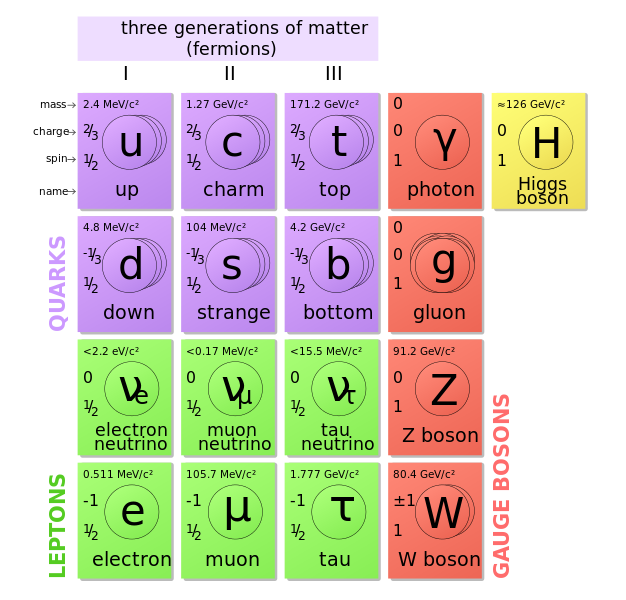
\includegraphics[width=1.00\columnwidth]{./figs/u01/standar-model-particles.png}}
		\column{0.45\textwidth}
    \begin{block}{Constituyentes}
			\begin{itemize}
        \color{chart01}{\item Materia}
        \color{chart09}{\item Interacciones}
        \color{chart07}{\item Masa}
        \item Parece inocente, pero:
			  \begin{itemize}
          \item $(6\cdot2)$ leptones = $12 l$
          \item $((6\cdot3)\cdot 2)$ quarks = $36 q$
          \item $(1+8+3+1)$ bosones = $13$ bosones de gauge
        \end{itemize}
        \item \bf{61 partículas ``fundamentales''}
      \end{itemize}
    \end{block}
  \end{columns}
\end{frame}

\begin{frame}
	\frametitle{Teorema de Noether}
  \framesubtitle{\alert{Simetrías de las ecuaciones $\leftrightarrow$ Cargas Conservadas}}
  \begin{block}{Simetrías}
			\begin{itemize}
        \item Invariancia rotaciones $\leftrightarrow$ Cons. momento angular
        \item Invariancia traslaciones espaciales $\leftrightarrow$ Cons. momento lineal
        \item Invariancia traslaciones temporales $\leftrightarrow$ Cons. Energía
			  \begin{itemize}
          \item Ver por ejemplo, Landau \& Lifshitz, Vol 1 (Mechanics, Cap II)
          \item Para simetrías, caldo Knorr, Landay \& Lifshitz, Vol 3 (Quantum Mechanics, Non-Relativistic Theory, Cap XII)
        \end{itemize}
        \item ¡Cuidado! Dice ``simetría de las ecuaciones'', no del problema $\rightarrow$ un cuerpo en rotación puede no tener un sólo eje de simetría pero conserva el impulso angular
      \end{itemize}
    \end{block}
    \begin{alertblock}{\centering{Las ecuaciones de movimiento son simétricas $\leftrightarrow$ hay cargas conservadas}}
  \end{alertblock}
  \begin{textblock*}{35mm}(90mm,0.00\textheight)
    \begin{exampleblock}{}
      {\centering 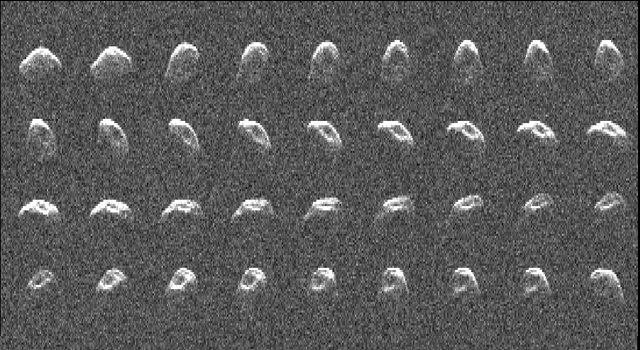
\includegraphics[width=1.00\columnwidth]{./figs/u01/asteroid-rotation.jpg}}
    \end{exampleblock}
  \end{textblock*}
\end{frame}

\begin{frame}
	\frametitle{Acción, simetrías y cargas}
  \framesubtitle{\alert{¿Que fue primero, el huevo o la gallina? ¿La conservación de la energía o la invariancia temporal?}}
  \begin{block}{Primero fue el huevo\ldots}
    \begin{itemize}
      \item Los principios de conservación se basan en observaciones de los sistemas naturales $\rightarrow$ {\bf{prejuicios}}
      \item \alert{Las ecuaciones movimiento, y por ende la acción, debe tener las simetrías necesarias para verificar las conservaciones observadas}
      \item Por ejemplo: {\color{chart04}{``La carga [eléctrica] es una magnitud conservada''}}
      \item Significa que nunca en la historia (es decir, {\bf{\emph{nunca hasta hoy y esperamos que eso no cambie -prejuicio-}}}) se observó un proceso donde la cantidad de carga eléctrica inicial y final difieren
    \end{itemize}
  \end{block}
  \begin{alertblock}{Moralejas}
    \begin{enumerate}
      \item Nuestra acción deberá incluir alguna simetría que, Noether mediante, contemple la conservación de la carga eléctrica
      \item \bf{La física es una ciencia natural, de carácter observacional y/o experimental $\rightarrow$ no es una ciencia ``exacta''}
    \end{enumerate}
  \end{alertblock}
\end{frame}

\begin{frame}
	\frametitle{Magnitudes conservadas}
  \begin{columns}
    \column{0.50\textwidth}
    {\centering 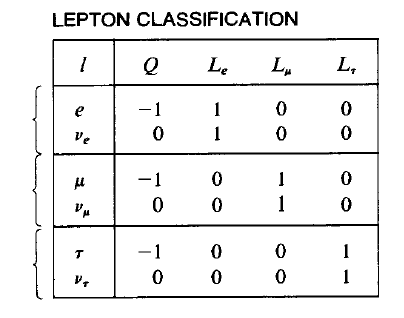
\includegraphics[width=1.00\columnwidth]{./figs/u01/lepton-number.png}}
    \begin{eqnarray*}
      p^+ \bar{\nu_e} &\rightarrow& n e^+ \qquad \alert{\mathrm{Si}}\\
      p^+ \nu_e &\rightarrow& n e^- \qquad \alert{\mathrm{No}}\\ 
      \mu^- &\rightarrow& e^- \bar{\nu_e} \nu_\mu \ \ \  \alert{\mathrm{Si}}\\ 
      p^+ \bar{\nu_\mu} &\rightarrow& n e^+ \qquad \alert{\mathrm{No}}\\
    \end{eqnarray*}
    \column{0.50\textwidth}
    \begin{block}{}
      \begin{itemize}
        \item Carga eléctrica
        \item Número leptónico por sabor (flavor)
        \item Las antipartículas tienen signos opuestos en todos los números
        \item Entonces, hay {\bf 12} leptones diferentes
        \item {\color{chart12}{\bf Los números antes y después de la reacción deben conservarse}}
      \end{itemize}
    \end{block}
  \end{columns}
\end{frame}

\begin{frame}
  \frametitle{QED (Quantum Electro Dynamics)}
  \framesubtitle{\alert{Electrodinámica cuántica (QED)}}
  teoría cuántica de campos (relativista) que describe las interacciones EM que ocurren entre partículas con carga eléctrica ($Q \neq 0$)
  \begin{alertblock}{Vértice fundamental}
    \begin{columns}
      \column{0.85\textwidth}
      \large{Diagramáticamente, el proceso elemental en QED puede representarse con el siguiente vértice:}
      \column{0.15\textwidth}
      {\hspace{-0.5cm}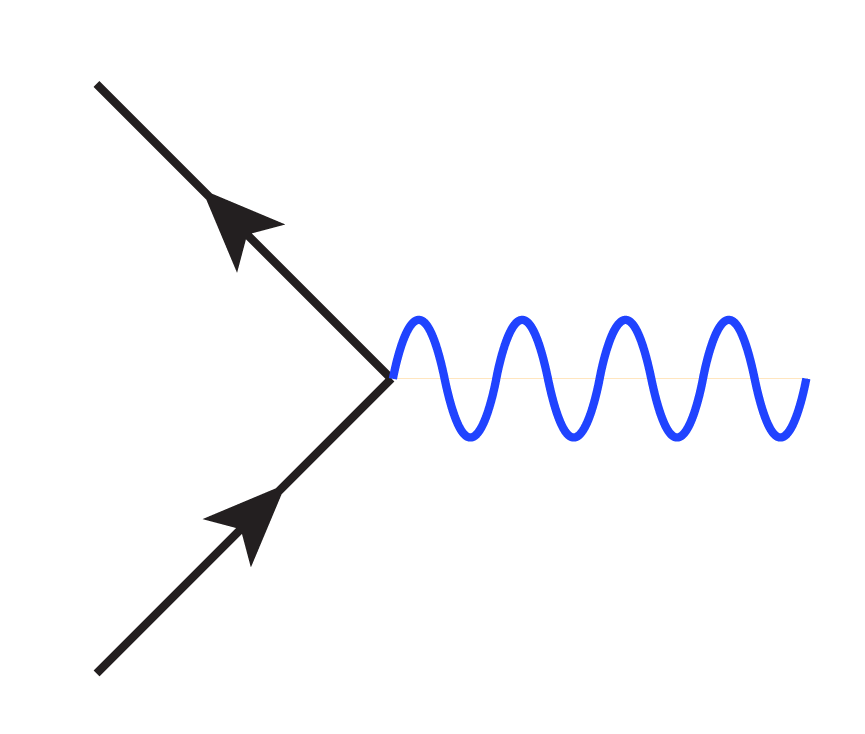
\includegraphics[width=1.15\columnwidth]{./figs/u01/qed-vertex.png}}
    \end{columns}
  \end{alertblock}
  \begin{block}{Convenciones diagramáticas}
    \begin{itemize}
      \item El tiempo se dibuja en dirección vertical sentido positivo hacia arriba
      \item La línea ondulada representa el intercambio de un fotón
      \item La flecha corresponde a una partícula cargada. Si la flecha apunta {\emph{contra}} el tiempo (sentido hacia abajo), representa a una antipartícula
      \item Los trazos no representan las trayectorias de las partículas
      \item {\bf \color{chart12}{En los vértices no pueden violarse las leyes de conservación}}
    \end{itemize}
  \end{block}
\end{frame}

\begin{frame}
  \frametitle{Infinitas contribuciones a un mismo estado}
  \begin{columns}
    \column{0.40\textwidth}
    {\centering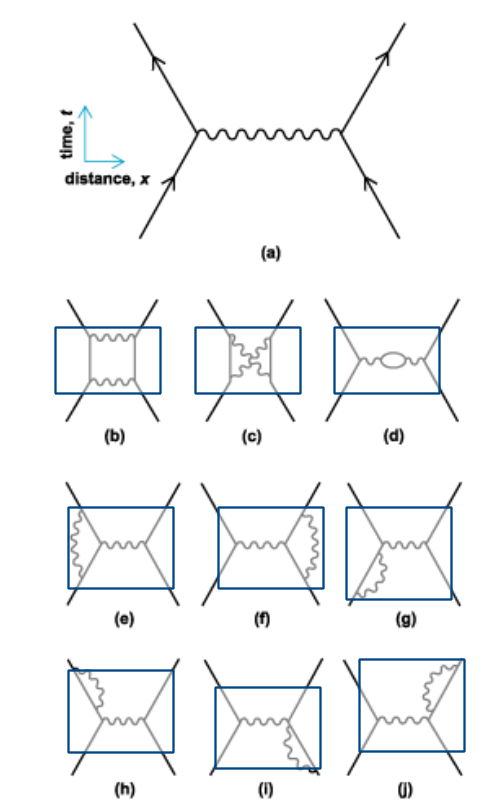
\includegraphics[width=1.0\columnwidth]{./figs/u01/qed-4vertex.png}}
    \column{0.60\textwidth}
    \begin{itemize}
      \item Todos estos procesos tienen el mismo estado asintótico: $e^- e^- \to e^- e^-$
      \item ¿Cuál de todos ellos ocurrió en realidad?
      \item Imposible saberlo $\rightarrow$ {\bf{\alert{ocurrieron todos}}} al mismo tiempo, y las {\bf{\color{chart09}{infinitas posibles combinaciones}}} también
      \item En QED, las contribuciones de cada estado al resultado final son cada vez más pequeñas (vértice $\sim \alpha_{\mathrm{EM}} \simeq 1/137$)
    \end{itemize}
  \end{columns}
\end{frame}

%%%%%%%%%%%%%%%%%%%%%%%%%%%%%%%%%%%%%%%%%%%
\section{Transformaciones de Lorentz}
%%%%%%%%%%%%%%%%%%%%%%%%%%%%%%%%%%%%%%%%%%%
\begin{frame}
  \frametitle{Transformaciones de Lorentz (TL ó Λ)}
  \begin{itemize}
    \item Grupo de Poincaré: Grupo de isometrías del espacio tiempo de Minkowsky
    \begin{itemize}
      \item Traslación temporal (1)
      \item Traslaciones espaciales (3)
      \item Rotaciones espaciales (3)
      \item Boosts espaciales (3)
    \end{itemize}
    \item Forman grupo frente a la composición de operaciones
    \begin{itemize}
      \item Hay una isometría “unidad” (no hago nada)
      \item existe la inversa (voy y vengo)
      \item son asociativas
    \end{itemize}
    \item Las transformaciones de Lorentz (Λ) son un subgrupo del grupo de Poincaré ($\mathbf{C}=\mathbf{0}_4$)
    \item Preservan el origen (invariante) → Rotaciones y Boosts
    \item Caldo Knorr\textregistered~ sobre Poincaré: se los consigo a pedido
  \end{itemize}
  \begin{textblock*}{38mm}(80mm,0.33\textheight)
    \large{
      \begin{equation}
        x'^\mu = x^\nu \Lambda^\mu_\nu+C^\mu
      \end{equation}
    }
  \end{textblock*}
\end{frame}

\begin{frame}
  \frametitle{Boosts}
  \begin{itemize}
    \item Transformaciones de Lorentz no rotantes: {\emph{cambios entre marcos de referencia incerciales}}
    \item Quedan definidos por el $\gamma$ de Lorentz (estrictamente $\beta \to \mathbf{\beta}=\mathbf{v}/c$)
    \item Puede demostrarse que un boost $\gamma$ en la dirección x puede expresarse como
    \begin{equation}
      \Lambda \equiv\Lambda_\nu^\mu = \left ( 
        \begin{array}{cccc}
          \gamma & -\beta\gamma & 0 & 0 \\
          -\beta\gamma & \gamma & 0 & 0 \\
          0 & 0 & 1 & 0 \\
          0 & 0 & 0 & 1
        \end{array}
      \right )
    \end{equation}
    \item Y luego, $S \to S'$
    \begin{equation}\label{EQboost}
      \left (
        \begin{array}{c}
          t' \\
          x' \\
          y' \\
          z' \\
        \end{array}
      \right ) 
      = 
      \left (
        \begin{array}{cccc}
          \gamma & -\beta\gamma & 0 & 0 \\
          -\beta\gamma & \gamma & 0 & 0 \\
          0 & 0 & 1 & 0 \\
          0 & 0 & 0 & 1
        \end{array}
      \right )
      \left (
        \begin{array}{c}
          t \\
          x \\
          y \\
          z \\
        \end{array}
      \right ) 
    \end{equation}
  \end{itemize}
\end{frame}

\begin{frame}
  \frametitle{\alert{Tarea 03-I (entrega en la clase 05)}}
  \begin{enumerate}
    \item Verificar que la ecuación (\ref{EQboost}) representa un boost de un sistema S' a un sistema S en la dirección $x$
    \item Escribir la transformación $\Lambda$ para un boost en la dirección $z$
    \item Verificar que los componentes de la (por ahora) matriz $\Lambda$ para una transformación general de Lorentz, $\mathbf{x'}=\Lambda \mathbf{x}$, representando un boost a un sistema con velocidad $\mathbf{v}=(\beta_1, \beta_2, \beta_3) c$ respecto al sistema de referencia, están dados por:
    \begin{eqnarray*}
      \Lambda_{00} &=& \gamma,\\
      \Lambda_{i0}=\Lambda_{0i} &=& -\beta_i \gamma,\\
      \Lambda_{ij}=\Lambda_{ji} &=& \delta_{ij} + (\gamma - 1) \frac{\beta_i \beta_j}{\beta^2}.
    \end{eqnarray*}
  \end{enumerate}
\end{frame}

\begin{frame}
	\frametitle{Ejemplo Real}
  \begin{columns}
    \column{0.50\textwidth}
    {\centering 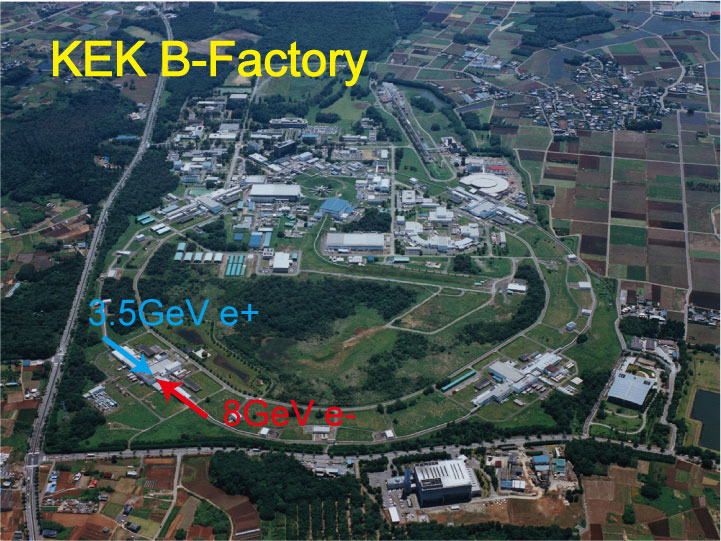
\includegraphics[width=1.00\columnwidth]{./figs/u01/kekb.png}}
    \column{0.50\textwidth}
    \begin{block}{KEK-B beam}
      \begin{itemize}
        \item Beam asimétrico
        \item Colisión $e^+ e^-$
        \item $E_{e^+} = 3.5$\,GeV
        \item $E_{e^-} = 8.0$\,GeV
        \item Boost del CM:
        \[ \beta \gamma = \frac{E_{e^-} - E_{e^+}}{\sqrt{4 E_{e^-} E_{e^+}}} \]
      \end{itemize}
    \end{block}
  \end{columns}
  \begin{exampleblock}{Tarea (continúa)}
    \begin{enumerate}\setcounter{enumi}{03}
      \item Con los valores especificados para las energías de cada beam, calcular la vida media $\tau$ del mesón $B$ en el marco del laboratorio (obtener la vida media $\tau_0$ del mesón $B$ del booklet). Luego, calcular la distancia recorrida por el mesón $B$ en el detector desde que es producido hasta que decae.
    \end{enumerate}
  \end{exampleblock}
\end{frame}

%%%%%%%%%%%%%%%%%%%%%%%%%%%%%%%%%%%%%%%%%%%
\section{Cálculo Tensorial}
%%%%%%%%%%%%%%%%%%%%%%%%%%%%%%%%%%%%%%%%%%%
\begin{frame}
	\frametitle{Cálculo Tensorial}
  \framesubtitle{Caldo Knorr\textregistered:~ Hernández\& Núñez, ``Métodos de Matemáticas Aplicadas'', Vol 1, Cap 3}
  \begin{itemize}
    \item Convención de Einstein en notación covariante: $\sum_{\mu=0}^3 x_\mu x^\mu \equiv x_\mu x^\mu$
    \item Índices latinos, $i,j,k,\ldots$: componentes espaciales ($1\ldots 3$),
    \item Índices griegos $\mu, \nu, \rho, \ldots$: espaciotemporales ($0\ldots 3$)
    \item Métrica de Minkowsky (plana), convención de signos usual en partículas, $\eta=(1,-1,-1,-1)$.
    \item El tensor métrico $g_{\mu\nu}$ queda entonces:
      \begin{equation}\label{EQmetrica}
        \mathbf{g} \equiv g_{\mu\nu} = \left ( 
          \begin{array}{cccc}
            1 & 0 & 0 & 0 \\
            0 & -1 & 0 & 0 \\
            0 & 0 & -1 & 0 \\
            0 & 0 & 0 & -1
          \end{array}
          \right ) = g^{\mu\nu}\equiv \mathbf{g}^{-1}
      \end{equation}
    \item Definimos {\bf{cuadrivector contravariante}} (cuadrivector) a un \alert{tensor contravariante de rango $1$}, que ante una transformación de Lorentz Λ se comporta como:
      \begin{equation}
        a'^\mu = \Lambda^{\mu}_{\nu} a^\nu
      \end{equation}
  \end{itemize}
  \begin{textblock*}{41mm}(84mm,0.38\textheight)
    \tiny 
    {
      \begin{exampleblock}{\tiny{Tarea (cont)}}
        \begin{enumerate}\setcounter{enumi}{04}
          \item Verficar que $\mathbf{g}\mathbf{g}^{-1} = g_{\nu\rho} g^{\mu\rho} = \delta^\mu_\nu$
          \item Verificar la relación de pseudo-ortogonalidad de las TL: \vspace{-2em}  
           \begin{equation}\label{EQorto}
             g_{\mu\nu} \Lambda^{\mu}_{\rho} \Lambda^{\nu}_{\sigma} = g_{\rho\sigma}
           \end{equation}\vspace{-3em}  
        \end{enumerate}
      \end{exampleblock}
    }
  \end{textblock*}
  \begin{textblock*}{41mm}(84mm,0.89\textheight)
    \Large{\alert{\bf{Cuadrivector}}}
  \end{textblock*}
\end{frame}

\begin{frame}
	\frametitle{cos y contras}
  \begin{itemize}
    \item Cada vector contravariante (vector) tiene asociado un vector covariante (forma), gracias a la métrica (contra $\to$ co)
      \begin{equation}
         (t,-\mathbf{r}) = a_\mu = g_{\mu\nu} a^\nu
      \end{equation}
    \item La transformación inversa co$\to$contra:
      \begin{equation}
        (t,\mathbf{r}) = a^\mu = g^{\mu\nu} a_\nu
      \end{equation}
    \item ¿Cómo transforma un vector covariante frente a una TL $\Lambda$?\\
      \begin{columns}
        \column{0.10\textwidth}
        \column{0.40\textwidth}
        \begin{eqnarray}
          a'_\mu &=& g_{\mu\nu} a'^\nu \nonumber\\ 
          a'_\mu &=& g_{\mu\nu} \Lambda^{\nu}_{\rho} a^\rho \nonumber\\
          a'_\mu &=& \underbrace{g_{\mu\nu} \Lambda^{\nu}_{\rho} g^{\rho\sigma}}_{\left ( \Lambda^{-1} \right )^\sigma_\mu} a_\sigma \nonumber
        \end{eqnarray}
        \vspace{-2em}
        \begin{alertblock}{}
          \begin{equation}
            a'_\mu = \left ( \Lambda^{-1} \right )^\sigma_\mu a_\sigma
          \end{equation}
        \end{alertblock}
        {\small{Queremos probar que el factor $g_{\mu\nu} \Lambda^{\nu}_{\rho} g^{\rho\sigma}$ es la TL inversa.}}
        \column{0.50\textwidth}
        {\small{Entonces recordamos (\ref{EQmetrica}) y (\ref{EQorto}):}}
        \begin{eqnarray}
          g_{\rho\theta} &=& g_{\mu\nu} \Lambda^{\nu}_{\rho} \Lambda^{\mu}_{\theta} \nonumber\\
          g_{\rho\theta} g^{\rho\sigma} &=& g_{\mu\nu} \Lambda^{\nu}_{\rho} \Lambda^{\mu}_{\theta}  g^{\rho\sigma} \nonumber \\
          \delta^{\sigma}_{\theta} &=& \underbrace{\left ( g_{\mu\nu} \Lambda^{\nu}_{\rho}  g^{\rho\sigma} \right )}_{\Xi^\sigma_\mu} \Lambda^{\mu}_{\theta} \nonumber \\
          \delta^{\sigma}_{\theta}  &=& \Xi_\mu^\sigma \Lambda^{\mu}_{\theta} \to \Xi_\mu^\sigma \left (\Lambda^{-1} \right )^\sigma_\mu \nonumber
        \end{eqnarray}
        \vspace{-2.0em}
        \begin{exampleblock}{}
          \begin{equation}
            \Rightarrow \left (\Lambda^{-1} \right )^\sigma_\mu = g_{\mu\nu} \Lambda^{\nu}_{\rho} g^{\rho\sigma}
          \end{equation}
        \end{exampleblock}
      \end{columns}
  \end{itemize}
  \begin{textblock*}{30mm}(6mm,0.70\textheight)
    \small{\alert{Si $\Lambda$ es un boost $\beta$, $\Lambda^{-1}$ es un boost $-\beta$}}
  \end{textblock*}
\end{frame}

\begin{frame}
  \frametitle{Tensores co y contravariantes}
  \begin{itemize}
    \item Un tensor de rango $n$ tendrá $n$ índices
    \item Transforman según $n$ TL:
      \[ F'^{\mu\nu} = \Lambda^{\mu}_{\rho} \Lambda^{\nu}_{\sigma} F^{\rho\sigma} \qquad \qquad 
      O'^{\mu\nu\theta} = \Lambda^{\mu}_{\rho} \Lambda^{\nu}_{\sigma} \Lambda^{\theta}_{\tau} O^{\rho\sigma\tau} \]
    \item Los hay también covariantes$\ldots$:
      \[ F'_{\mu\nu} = g_{\mu\rho} g_{\nu\sigma} F^{\rho\sigma} \]
    \item y $n$-co $m$-contra (el rango es $n+m$): 
      \[O_\mu^{\sigma\nu\theta} =  g_{\mu\rho} O^{\rho\sigma\nu\theta} \]
    \item Ver propiedades generales en Hernández\& Núñez, ``Métodos de Matemáticas Aplicadas'', Vol 1, Cap 3
  \end{itemize}
\end{frame}

\begin{frame}
\frametitle{(covariantes $\cdot$ contravariantes) $\to$ invariantes}
  \begin{itemize}
    \item Propuesta 1: \alert{La composición de dos TL es una TL}:
      \begin{eqnarray}
        a'^\mu &=& \Lambda^{\mu}_{\nu} a^\nu \qquad \mathrm{y} \qquad a''^\rho = \Lambda'^{\rho}_{\mu} a'^\mu \nonumber\\
        \to a''^\rho &=& \Lambda'^{\rho}_{\mu} \Lambda^{\mu}_{\nu} a^\nu \nonumber\\
        a''^\rho &=& \left (\Lambda' \Lambda \right)^{\rho}_{\nu} a^\nu \nonumber\\
        a''^\rho &=& \Lambda''^{\rho}_{\nu} a^\nu
      \end{eqnarray}
    \item Propuesta 2: \alert{El producto escalar $\mathbf{a}\cdot\mathbf{b}\equiv a_\mu b^\nu = a^\mu b_\nu$ es invariante ante transformaciones de Lorentz}:
      \begin{eqnarray}
        \mathbf{a'} \cdot \mathbf{b'} &=& a'_\mu b'^\mu \nonumber\\
        \mathbf{a'} \cdot \mathbf{b'} &=& (\Lambda^{-1})_\mu^\sigma a_\sigma \Lambda_\rho^\mu b^\rho \nonumber\\
        \mathbf{a'} \cdot \mathbf{b'} &=& (\Lambda^{-1})_\mu^\sigma \Lambda_\rho^\mu a_\sigma  b^\rho \nonumber\\
        \mathbf{a'} \cdot \mathbf{b'} &=& \delta^\sigma_\rho a_\sigma b^\rho \nonumber\\
        \mathbf{a'} \cdot \mathbf{b'} &=& a_\rho b^\rho = \mathbf{a} \cdot \mathbf{b}
      \end{eqnarray}
  \end{itemize}
\end{frame}

\begin{frame}
  \frametitle{Tres invariantes famosos tres}
  \begin{itemize}
    \item \alert{Invariante $ds^2$}:
      \begin{equation}
        ds^2 \equiv dx^\mu dx_\mu = d(ct)^2 - (dx)^2 - (dy)^2 - (dz)^2
      \end{equation}
    \item \alert{Derivadas parciales}:
      \begin{equation}
        \frac{\partial}{\partial^\mu} \equiv \partial_\mu = \left( \frac{\partial}{\partial t}, \nabla \right)
        \qquad \mathrm{y} \qquad
        \frac{\partial}{\partial_\mu} \equiv \partial^\mu = g^{\mu\nu} \partial_\nu = \left(\frac{\partial}{\partial t}, -\nabla \right)
      \end{equation}
      y luego, el invariante es el operador \alert{D'alambertiano}:
      \begin{equation}
        \partial_\mu \partial^\mu = \left(\frac{\partial^2}{\partial t^2} - \nabla^2 \right) \equiv \square
      \end{equation}
    \item \alert{Cuadrivector Energía-momento}: Recordando clase 01-01: $E=\gamma m_0$ y $\mathbf{p}=\gamma m_0 \mathbf{v}$, podemos formar un cuadrivector:
      \begin{equation}
        p^\mu \equiv (E,\mathbf{p}) \qquad \mathrm{y} \qquad  p_\mu = g_{\mu\nu} p^\nu \equiv (E,-\mathbf{p})
      \end{equation}
      y luego, contrayendo, obtenemos uno de los invariantes más importantes:
      \begin{alertblock}{
          \begin{equation}
            p^\mu p_\mu = E^2 -\mathbf{p}^2 = m_0^2
          \end{equation}
      }
    \end{alertblock}
  \end{itemize}
\end{frame}

\begin{frame}
  \frametitle{\alert{Tarea 03 (último)}}
  \begin{enumerate}\setcounter{enumi}{04}
    \item Verificar explicitamente que $p^\mu p_\mu$ es un invariante ante TL
    \item Griffiths: leer sección 3.4, para discutir en clase 04
    \item Griffiths: problemas 3.4, 3.11, 3.12, 3.14, y alguno del 3.15
  \end{enumerate}
\end{frame}

\end{document}
